\section{Introduction}

In this lab, our goal is to study the phenomenon of simple harmonic oscillation,
find the spring constant and effective mass of a spring,
and how to use the air track. We will analyze the relationship between the
oscillation period and the mass of the oscillator, check whether the oscillation
period depends on the the amplitude, and examine the relationship between the
maximum speed and the amplitude. 

There are various kinds of periodic motion in nature, among which the simplest
and the most fundamental one is the simple harmonic motion, where the restoring
force is proportional to the displacement from the equilibrium position and as a
result, the position of a particle depends on time as the sine (or cosine)
function. Discussion of the simple harmonic motion is a basis for studying more
complex situations. 

\subsubsection{Hooke's Law}
Within the elastic limit of deformation, the force Fx needed to be applied in
order to stretch or compress a spring by the distance x is proportional to that
distance, i.e.

\begin{equation}
\label{hookeslaw}
F_x=kx,
\end{equation}

where $k$ is a the spring constant that characterizing how easy it is to deform a
spring.
This constant will be found in the present exercise using a measurement device
called the Jolly balance. 
The linear relation  between the force and the deformation, is known as the
Hooke’s Law.
According to Newton's third law of dynamics, the spring exerts a reaction force
(called the elastic force) of the same magnitude but opposite direction. 

\subsection{Equation of Motion of the Simple Harmonic Oscillator}
\begin{figure}[H]
\centering
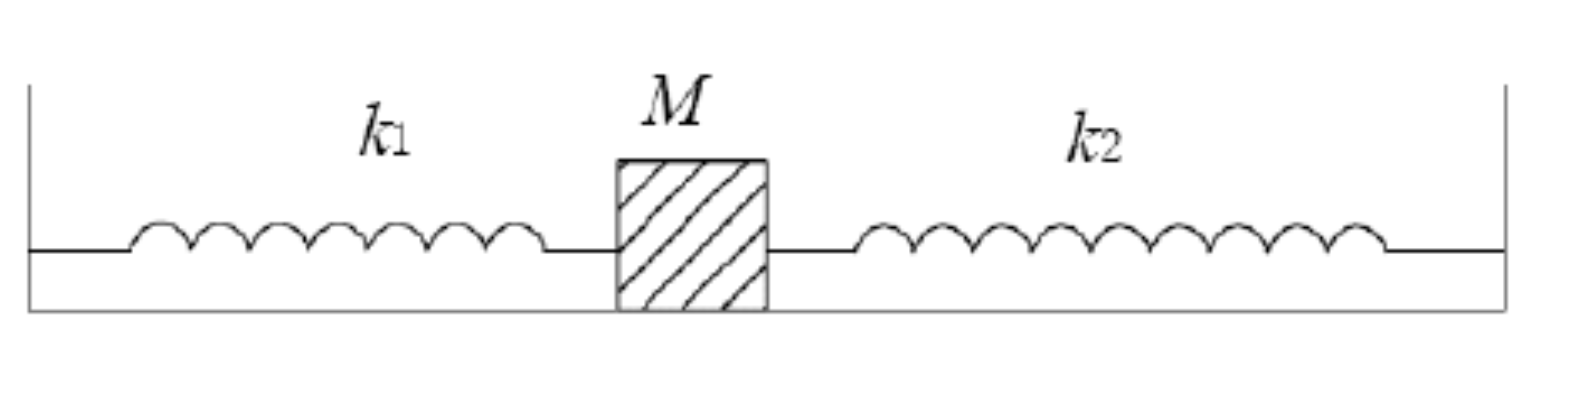
\includegraphics[width=12cm]{fig/i1}
\caption{Mass-spring system}
\label{mss}
\end{figure}

As shown in Figure~\ref{mss}, the mass with two springs is placed on an
air track, which aims at eliminating the frictional forces. Assuming that the
restoring force is the only force acting on mass M, the equation of motion od
mass M is 

\begin{equation}
\label{M1}
M\frac{d^2x}{dt^2}+(k_1+k_2)x=0.
\end{equation}

Hence the general solution to Eq. \ref{M1} is

\begin{equation}
x(t)=Acos(\omega_0t+\phi_0),
\end{equation}

where $\omega_0=\sqrt{(k_1+k_2)/M}$ is the natural angular frequency of the
oscillations (determined by the parameters of the system), A is the amplitude,
and $\phi_0$ is the initial phase (determined by initial conditions). The
natural period of oscillation is 

\begin{equation}
T=\frac{2\pi}{\omega_0}=2\pi\sqrt{\frac{M}{k_1+k_2}}.
\end{equation}
    
In this exercise, the relationship mentioned above will be studied.
    
\subsection{Mass of the Spring}

We take into the mass of the springs in terms of the so-called
effective mass, which is the sum of the mass of the object $M$ and
the effective mass of springs $m_0$.
The angular frequency can be expressed as

\begin{equation}
  \label{omega1}
\omega_0=\sqrt{\frac{k_1+k_2}{M+m_0}}
\end{equation}

where $m_0$ is 1/3 of the actual mass of the spring.

\subsection{Mechanical Energy in Harmonic Motion}

The elastic potential energy for a spring-mass system is $U=kx^2/2$ and the
kinetic energy of an oscillating mass is $K=mv^2/2$.
At the equilibrium position ($x=0$), the speed of the mass is maximum
$v=v_{\max}$. 
At this point the total mechanical energy is equal to maximum kinetic energy
$K_{\max}$ . 
On the other hand, at maximum displacement ($x=\pm A$) the mass is
instantaneously at rest, and the contribution to the total mechanical energy is
due to the potential energy only, which is at its maximum $U_{\max}$. 
In the absence of non-conservative forces (such as frictional forces or drag
forces), the total mechanical energy is conserved and $K_{\max}=U_{\max}$, which
implies  

\begin{equation}
k=\frac{m (v_{max})^2}{A^2}
\label{kmv2_A2}
\end{equation}

